%第4章:検証
%結果(実験で起こったこと)を書く.客観的に.グラフあればなおよし.


\section{検証}


\subsection{詳細設計の検証}

まず,各種センサが要件を満たすかどうか検証した.

\subsection*{Webカメラ}

対象商品をカメラから100mm,150mm,200mmと離し,バーコードを読み取れるかテストを行った.カゴの高さが240mmかつ,Webカメラの設置場所はカゴの上部90mmのため,150~200mm程度までバーコードが認識できれば構わないとする.

はじめに,WebカメラとしてロジクールC270を使用し,テストを行った.全て画像のピントが合っておらず,バーコードを読み取ることができなかった.より画質が高く,ピントの合いやすいスマートフォンのカメラで撮影した動画でバーコード読み取りを試したところ,100mm,150mm程度まで読み取ることができたため,バーコード読み取りシステムの不具合ではなかったことが判明した.画素数もしくはピントを合わせる機能が問題になっていると仮定した.

次に,Raspberry Pi カメラモジュール V2を使用し,テストを行った.Raspberry Pi カメラモジュール V2については画素数はロジクールC270の約6.6倍の画素数のため,もし画素数に問題があるならば判明すると考えた.Raspberry Pi カメラモジュール V2をテストしたところ,ロジクールC270と同じようにピントが合わず,バーコードを読み取ることができなかった.

画素の問題でないことが判明したため,オートフォーカスモデルのロジクールC615を使用しテストを行った.バーコードの読み取り距離について要求を満たしたため,表\ref{jissou}に最終的な実装環境として,ロジクールウェブカメラC615を記載した.

\subsection*{超音波センサ}

超音波センサが正しく反応しているか,要求を満たしているかテストを行った.要求としてはカゴの横幅360mmなので,360mm以内を10mm程ずつ測ることができるかどうか確認した.超音波センサは正しく反応し,360mm以上の距離を1mmより小さい距離ずつ測ることができ,要求を満たした.

\subsection*{ロードセル}

ロードセルが正しく反応しているか,要求を満たしているかテストを行った.要求として,重量の増減を確認できるか,3kgまでの重量を1g程ずつはかることができるかどうか確認した.ロードセルは正しく反応し,対象商品を1gより小さい値ずつ測ることができた.そのためロードセルは要求を満たした.

\subsection*{LED}

LEDが正しく点灯するかどうか確認した.各LEDを抵抗と共にブレッドボードに設置し,点灯するかテストしたところ,正しく点灯した.


\subsection{単体テスト}

V字モデルに従い,詳細設計を満たしているかどうかを確認する.各実装対象の単体テストの内容を表\ref{tantai}に示す.

\begin{figure}[htbp]
\centering
\caption{単体テスト}
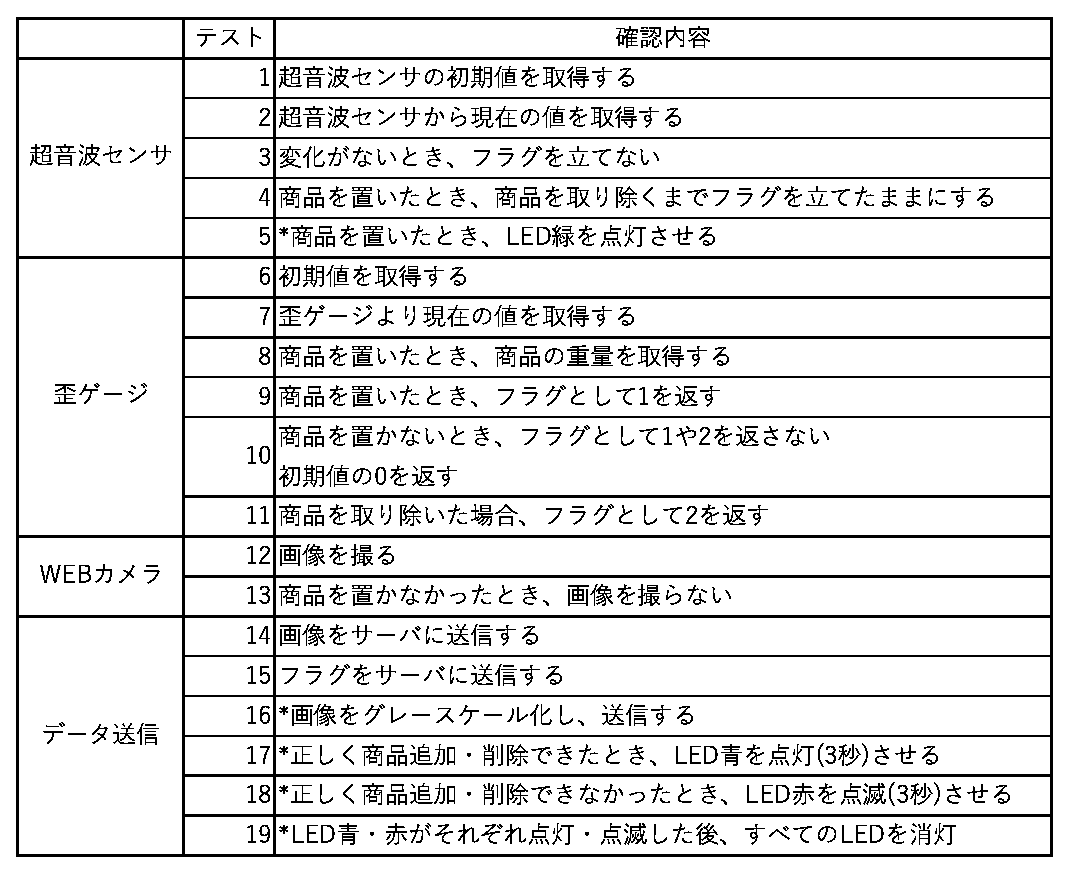
\includegraphics[width = 15cm]{./picture/tantai.eps}
\label{tantai}
\end{figure}

\subsection{結合テスト}


\subsection{総合テスト}
